%
\comment{

1. For this paper, we design and evaluate for a specific and common application
--> allows for comparison to previous work (Brebner)
2. Describe architecture of processing modules
3. Describe processing features of each processing module
4. Describe data path width and frequency
>> Describe process of packets how they traverse the processor 
5. Show how duplication of modules allows for the support of higher bandwidth
6. Show how using both directions of the NoC can double supported BW
7. Highlight customizability of this design
- new protocols can be added
- more modules can be added to support more throughput
- some protocols don't have to be duplicated as much if we know that there traffic is low (see evaluation section)

}
%

In order to evaluate this design, we implemented a packet processor that supports processing of several common network protocols: Ethernet, VLAN, IPv4, IPv6, and TCP.
Table~\ref{tbl:proc} lists the features implemented in each of the protocol processing modules.
%Each of the processing modules follows a similar architecture.
%Packets arriving at the modules are sent through pipeline registers, while module-specific logic performs the processing functions in parallel.
Each packet going through the processor will visit a processing module for each protocol found in its header.
For example, consider an Ethernet/IPv4/TCP packet.
The packet is first brought onto the chip through the FPGA's transceivers, which perform clock recovery and serial to parallel data conversion.
It is then transported to the embedded NoC through the FPGA's soft interconnect, where the FabricPort (Section~\ref{sec:noc-fpga}) performs clock conversion to bring the data from the slower FPGA fabric to the fast NoC.
The NoC's links and routers steer the packet to a router connected to an Ethernet processing module, where the FabricPort again performs clock conversion to bring the packet back to the FPGA fabric.
Once Ethernet processing is complete and the next layer protocol is determined, the packet is then brought back to the NoC to be sent to an IPv4 processing module, and finally a TCP processing module, before being sent back out through the FPGA's transceiver.

%The number of pipeline registers implemented is equal to the number of processing cycles required before the packet can be sent.

%
%
\begin{table}[!t]
\centering
\begin{small}
    \caption{Functions implemented in each protocol processing module in our NoC-PP design.}
    \label{tbl:proc}
    \begin{tabular}{ll}
    \toprule
    \textbf{Protocol} & \textbf{Implemented Processing Functions} \\
    \textbf{Module} &  \\
    \midrule
	Ethernet/VLAN & 1. Parse MAC source and destination   \\ 
	              & 2. Maintain a MAC table with address-port \\
	              &    mappings \\
	              & 3. Extract priority code identifier (PCP) in \\
	              &    VLAN header \\
	              & 4. Determine layer 3 protocol from Ethertype \\
	\midrule
	IPv4          & 1. Compute checksum and drop packet if  \\
	              &    results in error    \\
	              & 2. Decrement time to live (TTL) and drop \\
	              &    packet if zero reached\\
	              & 3. Determine total length of header \\
	              & 4. Parse source and destination IP addresses \\
	              & 5. Determine layer 4 protocol \\
	\midrule
    IPv6          & 1. Decrement hop limit and drop packet if \\
    			  &    zero reached   \\
    			  & 2. Parse source and destination IP addresses \\
    			  & 3. Determine layer 4 protocol \\
    \midrule
    TCP           & 1. Parse source and destination ports    \\
    			  & 2. When receiving a request to establish a \\
    			  &    connection, generate and send a reply ACK \\
    			  &    message over TCP/IP \\
    \bottomrule
    \end{tabular}
\end{small}
\end{table}
%
%

%\figvs{1}{processing-module}{}{General architecture of processing modules in NoC-PP.}

%
\begin{figure*}
\centering
%
        \begin{subfigure}[t]{0.45\textwidth}
        		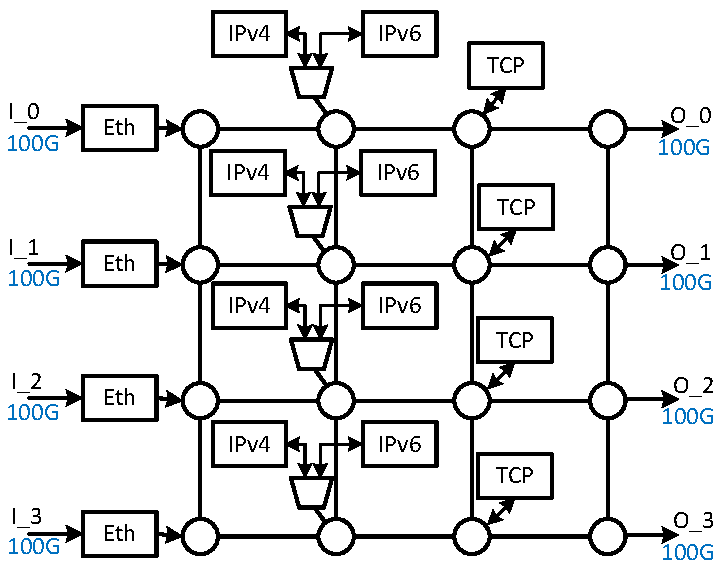
\includegraphics[width=\textwidth]{figs/noc-pp-uni.pdf}
        		\caption{400G}
        		\label{400g}
		\end{subfigure}
        \begin{subfigure}[t]{0.45\textwidth}
        		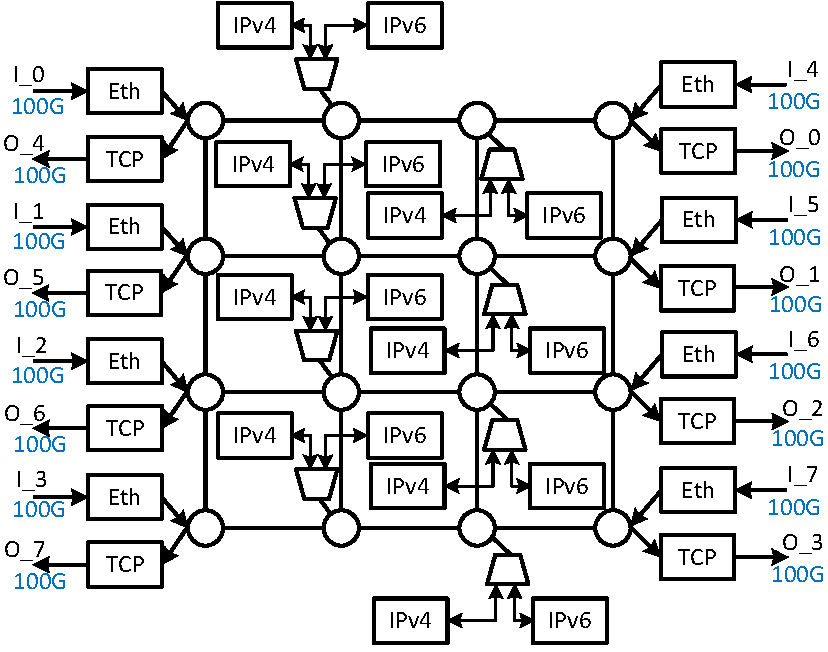
\includegraphics[width=\textwidth]{figs/noc-pp-bi.pdf}
        		\caption{800G}
        		\label{800g}
		\end{subfigure}
\caption{The NoC PP design for an Ethernet/VLAN/IPv4/IPv6/TCP packet processor (Eth=Ethernet+VLAN). Processing modules run at 100G, and are instantiated four times to support 400G processing, or eight times to support 800G processing.}
\label{noc-pp}
\end{figure*}
%

The processing modules are designed with a data path width of 512 bits running at 200 MHz, providing an overall processing throughput of 100 Gb/s.
There are two possible ways for this design to support a higher network bandwidth: increase the supported throughput of the individual processing modules or instantiate multiple instances of the processing module throughout the NoC.
In our design, we duplicate the 100G processing modules to provide higher overall processing bandwidths, such as 400G and 800G (Figure~\ref{noc-pp}).
This ability to duplicate individual processing modules provides a key form of design flexibility not found in previously proposed packet processor designs.
If a designer is aware of the expected frequencies of traffic of each of the different protocols, then he/she can duplicate the different processing modules to the appropriate degree.
For example, if IPv4 packets are currently much more frequent compared to IPv6 packets, then the design could instantiate more IPv4 processing modules than IPv6.
This design flexibility is explored in Section~\ref{sec:flex}.

Besides module duplication, the NoC-PP design also allows for the easy addition and/or removal of protocols, thanks to the logical and physical decoupling of processing modules by the NoC.
Say a new protocol has been developed and must be supported by the packet processor.
A processing module for this protocol can then be designed and added to the NoC-PP by connecting it to any of the routers in the NoC, with little other modification to the rest of the design.
Similarly, if a protocol no longer needs to be supported, then its processing modules can simply be removed from the design.

